\documentclass[11pt]{article}

% ---------------------------------------------------------------------------
% Endpoint-precision note --- the two-scanner study: the distal-edge estimator
% and its precision on the two representative CRYSP configurations (BGO 195 K
% and cryogenic CsI, same ring, 2 X0 crystals). British spelling.
% Compile: tools/latex_compile.py endpoint_precision
% Figures from the output tree are collected by tools/collect_note_figures.sh
% ---------------------------------------------------------------------------

\usepackage[T1]{fontenc}
\usepackage[utf8]{inputenc}
\usepackage[british]{babel}
\usepackage[a4paper,margin=2.5cm]{geometry}
\usepackage{graphicx}
\usepackage{booktabs}
\usepackage{siunitx}
\usepackage{amsmath}
\usepackage[numbers,sort&compress]{natbib}
\usepackage[hidelinks]{hyperref}
\usepackage{amssymb}

\sisetup{detect-all}
\newcommand{\Rfifty}{R_{50}}
\newcommand{\DR}{\Delta R}

\title{Precision of $\beta^+$ distal-edge verification:\\
  the two representative CRYSP scanners}
\author{J.J. G\'omez-Cadenas}
\date{\vspace{-3em}}

\begin{document}
\maketitle

\begin{abstract}
We quantify the precision with which an in-room PET scanner determines the
distal edge of a proton field from the $\beta^+$ activity it induces, for
the two representative CRYSP configurations: BGO at \SI{195}{K} and
cryogenic CsI, on the same closed \SI{1}{m} ring with two-radiation-length
crystals. Each scanner is simulated as ten independent \SI{1}{Gy}
acquisitions of an SOBP field in a head phantom, reconstructed with the
full list-mode chain. The estimator --- the midpoint $\Rfifty$ of the
distal activity fall-off, fitted on the whole-plane depth profile --- is
established with its calibration budget per arm, each term resolved to
\SIrange{0.01}{0.04}{mm}. The headline is a tie: at the realistic protocol
(all events, no corrections) both scanners measure the edge with
$\sigma_R = 0.11\,$mm per \SI{1}{Gy} acquisition --- BGO's $2.1\times$
statistics cancels against its $2.1\times$ scatter fraction. On true
coincidences the arms separate ($0.065$ vs.\ \SI{0.084}{mm}), which is the
margin a scatter correction would unlock. The precision follows
$1/\sqrt{\text{dose}}$ with a dose-invariant calibration on both arms, so a
\SI{0.1}{Gy} exploratory shot locates the edge to
\SIrange{0.16}{0.23}{mm} before the clinical dose is delivered.
\end{abstract}

\section{Setup}
\label{sec:setup}

The study case is an SOBP proton field depositing a uniform \SI{1}{Gy} in a
head phantom: an ellipsoid of uniform brain tissue with semi-axes
$(72, 87, 102)$\,mm (the beam axis is $z$). The nuclear interactions of the
protons produce $\beta^+$ emitters along the beam path --- mainly $^{15}$O
($T_{1/2}=\SI{122}{s}$) and $^{11}$C (\SI{20.4}{min}), with $^{13}$N,
$^{10}$C and $^{14}$O contributions --- whose annihilation photons the
scanner images. Figure~\ref{fig:sobp} shows the two nominal curves of the
problem: the depth--dose $D(z)$ and the depth profile of the $\beta^+$
activity $A(z)$. Because isotope production requires protons above the
reaction thresholds ($\approx 17$ and \SI{18}{MeV} for the main $^{15}$O
and $^{11}$C channels), the activity ends about \SI{11}{mm} upstream of the
dose edge. That offset is stable beam physics: it is what a simulation
calibrates and a measurement rides on.

\begin{figure}[htb]
  \centering
  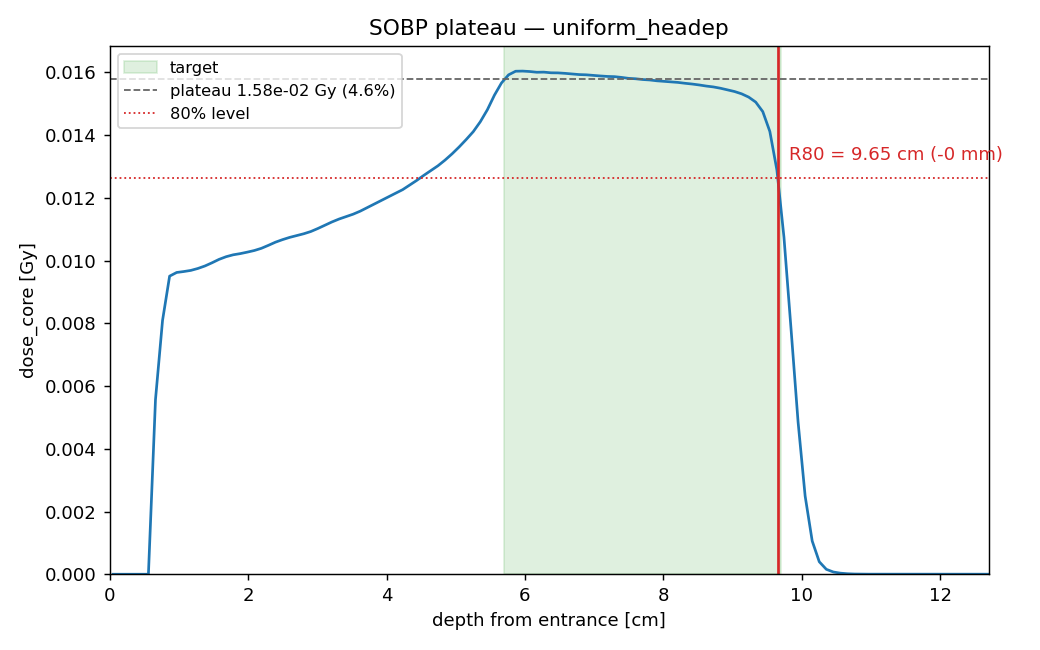
\includegraphics[width=0.46\textwidth]{figs/sobp_plateau.png}
  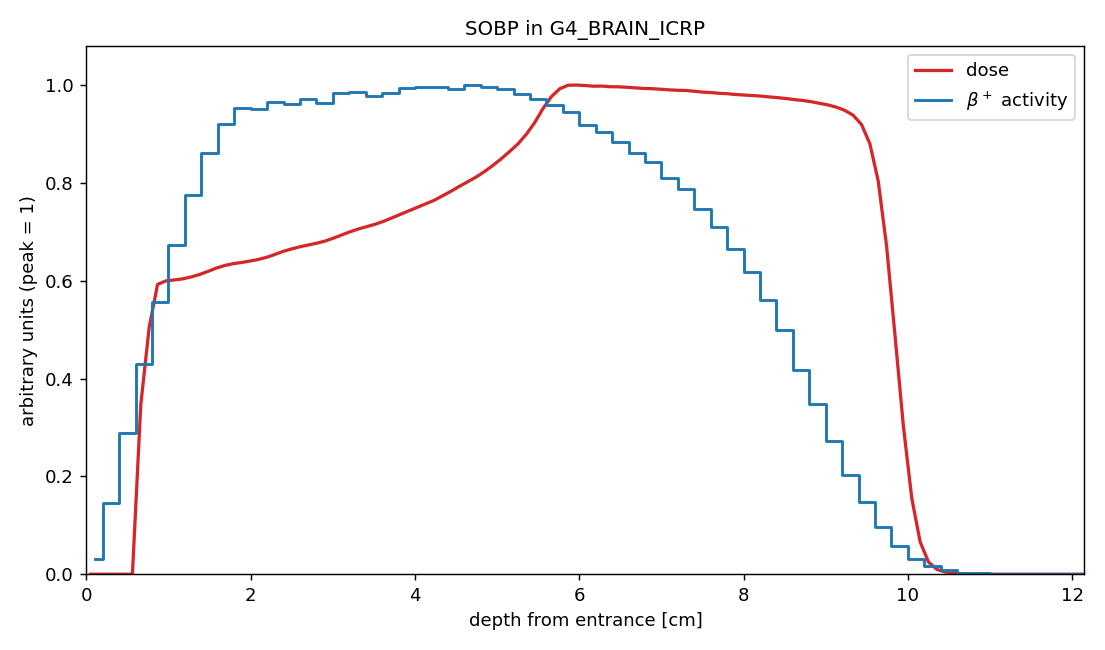
\includegraphics[width=0.46\textwidth]{figs/dose_activity.png}
  \caption{Left: the SOBP depth--dose and the definition of the clinical
    range point $R_{80}$. Right: the nominal $\beta^+$ activity profile
    together with the dose profile; the activity edge sits $\approx
    \SI{11}{mm}$ upstream of the dose edge, set by the production
    thresholds.}
  \label{fig:sobp}
\end{figure}

\subsection*{The two scanners}

Both configurations are the same closed cylindrical ring --- inner radius
\SI{387}{mm}, axial length \SI{1024}{mm}, $48\times20$ monolithic blocks
--- differing only in crystal, each at a depth of \textbf{two radiation
lengths} (the standard on which the CRYSP position resolution of
\SI{3.5}{mm} FWHM per axis is measured). Table~\ref{tab:arms} gives the
detector constants and the resulting per-acquisition statistics; the
timing windows come from the calibrated CTR model of the production
campaign, anchored to the cryogenic CsI bench measurement
of ref.~\cite{soleti_csi}.

\begin{table}[htb]
  \centering
  \caption{The two arms. Shared: ring geometry, position resolution
    $\sigma_{xyz} = \SI{1.486}{mm}$ (\SI{3.5}{mm} FWHM), acquisition window
    \SIrange{0}{1200}{s}, and the annihilation sets (acquisition $R$ sees
    identical decays on both scanners --- differences are detector-only).
    Statistics are per \SI{1}{Gy} acquisition ($8.02\times10^{7}$ decays).}
  \label{tab:arms}
  \vspace{1mm}
  \begin{tabular}{lcc}
    \toprule
     & BGO (\SI{195}{K}) & CsI (${\sim}\SI{100}{K}$) \\
    \midrule
    crystal depth ($2X_0$)            & \SI{22.4}{mm} & \SI{37.2}{mm} \\
    energy resolution (FWHM, 511 keV) & 15\%          & 6\%  \\
    photopeak cut ($511 - 3\sigma_E$) & \SI{413}{keV} & \SI{472}{keV} \\
    coincidence window $\tau$         & \SI{5}{ns}    & \SI{1.5}{ns} \\
    \midrule
    coincidences                      & $15.3\times10^{6}$ & $6.1\times10^{6}$ \\
    true / scatter / random           & $72.3\,/\,27.4\,/\,0.3\%$
                                      & $86.6\,/\,13.3\,/\,0.1\%$ \\
    \bottomrule
  \end{tabular}
\end{table}

The contrast is the point of the pair: BGO delivers $2.1\times$ the true
coincidences; CsI delivers purity --- half the scatter fraction and
$3\times$ fewer randoms from its energy resolution and timing. The range
measurement arbitrates between them.

Images are reconstructed with list-mode MLEM~\cite{shepp_vardi} on a
$64\times64\times96$ grid of \SI{1.5}{mm} voxels covering the activity
corridor, with 50 iterations, per-event attenuation factors computed
analytically on the phantom ellipsoid, and a per-arm sensitivity image from
$10^{9}$ sampled lines of response. Figure~\ref{fig:projections} shows the
orthogonal projections of one reconstructed BGO acquisition; the CsI image
is identical in geometry, with $2.1\times$ fewer counts.

\begin{figure}[htb]
  \centering
  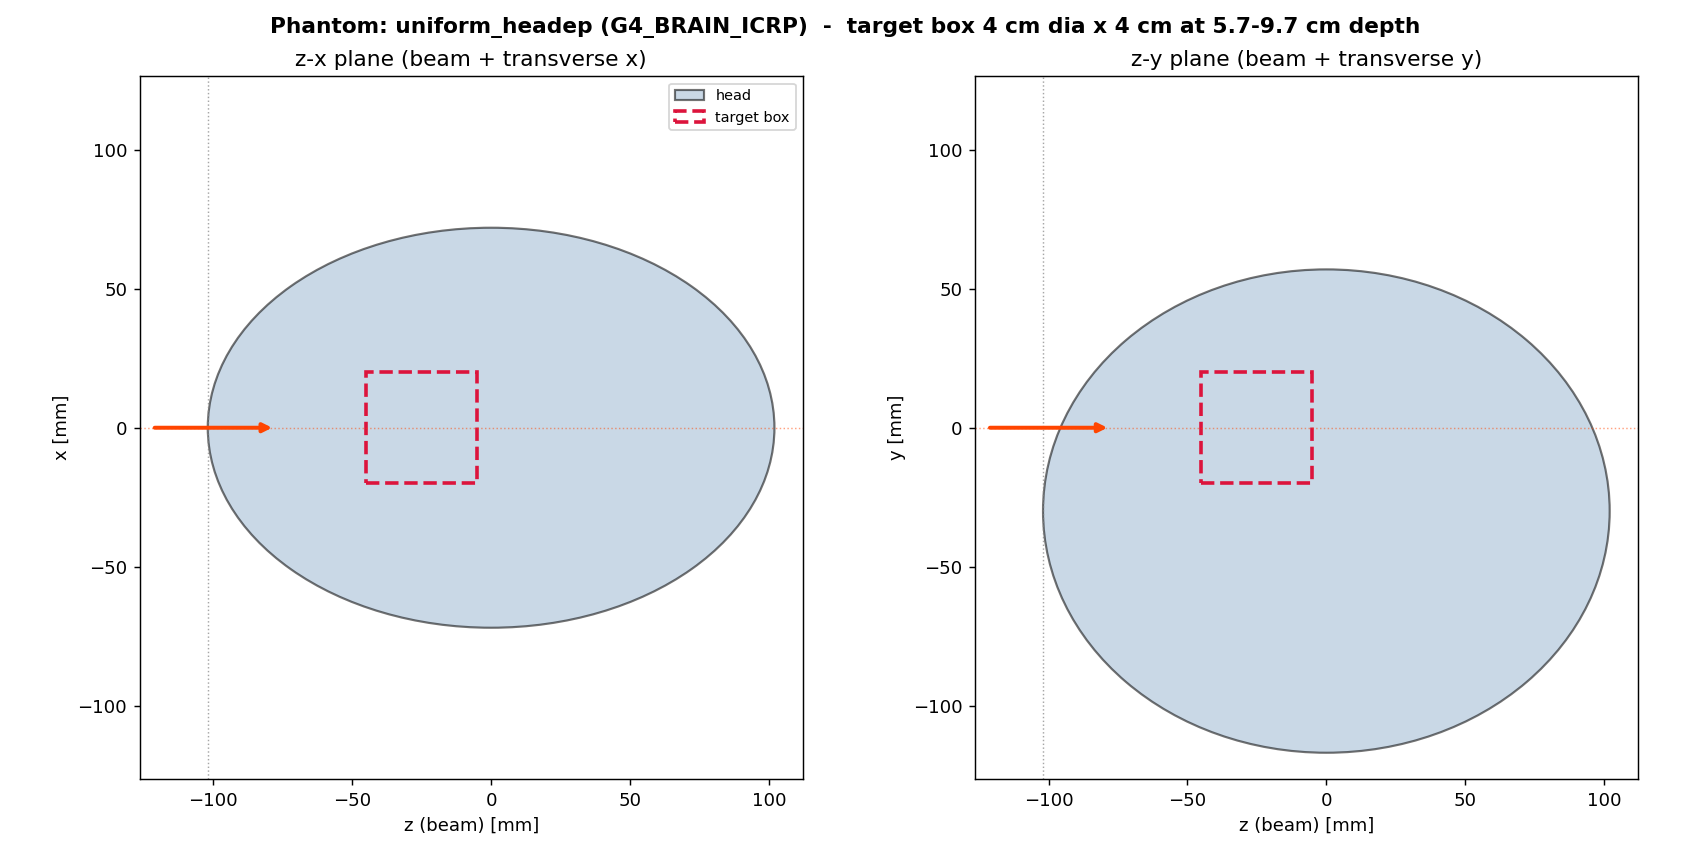
\includegraphics[width=0.55\textwidth]{figs/phantom.png}\\[2mm]
  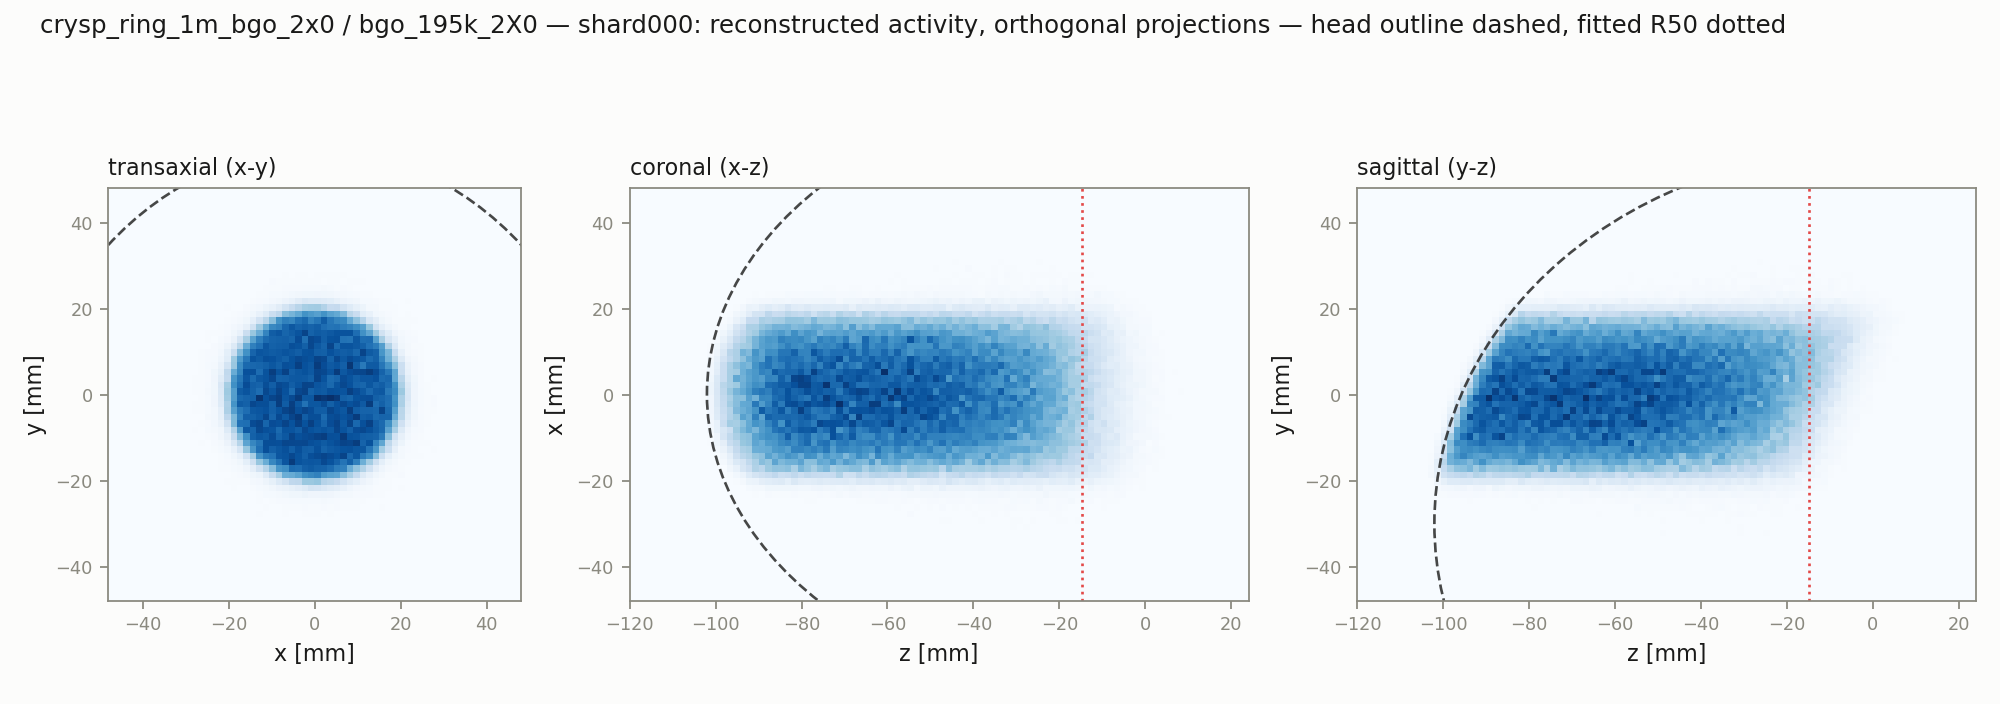
\includegraphics[width=\textwidth]{figs/recon_projections_bgo.png}
  \caption{Top: the head phantom, an ellipsoid of uniform brain tissue.
    Bottom: orthogonal projections of the reconstructed activity of one
    \SI{1}{Gy} BGO acquisition (transaxial, coronal, sagittal). The dashed
    curve is the phantom outline; the dotted line marks the fitted
    $\Rfifty$.}
  \label{fig:projections}
\end{figure}

\section{The estimator}
\label{sec:estimator}

The depth profile is the activity integrated over the full transverse
plane at each depth,
\begin{equation}
  P(z) \;=\; \iint A(x,y,z)\,\mathrm{d}x\,\mathrm{d}y ,
  \label{eq:profile}
\end{equation}
which makes the profile insensitive to the transverse spreading of the beam
with depth. The distal fall-off is fitted with a complementary error
function plus a baseline,
\begin{equation}
  P(z) \;=\; b + \frac{a}{2}\,
  \operatorname{erfc}\!\left(\frac{z - z_0}{\sqrt{2}\,w}\right),
  \label{eq:erfc}
\end{equation}
inside a fixed window bracketing the edge ($-36.5 \le z \le \SI{-1.5}{mm}$
for the nominal beam), with Poisson weights. The four parameters are the
baseline $b$, the plateau amplitude $a$, the midpoint $z_0$ and the edge
width $w$.

\paragraph{Range points.} For any curve with a plateau and a distal
fall-off, $R_X$ denotes the depth at which the curve has dropped to $X\%$ of
its plateau. Two of them play distinct roles:
\begin{itemize}
\item $\Rfifty \equiv z_0$, the \emph{midpoint} of the fall-off, is the
  range observable. It is where the profile is steepest, so it carries the
  smallest statistical error of any level, and Eq.~(\ref{eq:erfc}) yields it
  directly as a fit parameter.
\item $R_{80}$ of the \emph{dose} is the clinical prescription point
  (Fig.~\ref{fig:sobp}, left). For a given beam it differs from the dose
  $\Rfifty$ by a fixed geometric constant of the SOBP shape
  ($R_{80}-\Rfifty^{\text{dose}} = \SI{-2.0}{mm}$ for the nominal beam), so
  a measurement expressed in $\Rfifty$ converts to $R_{80}$ exactly.
\end{itemize}

\paragraph{The $\DR$ estimator.} The measured quantity is
\begin{equation}
  \DR \;=\; \Rfifty^{\text{activity}} - \Rfifty^{\text{dose}},
  \label{eq:dr}
\end{equation}
with the same fit construction, Eq.~(\ref{eq:erfc}), applied to both
curves. $\DR$ is calibrated once on the reference simulation of the
treatment plan --- per scanner, since the constant is a property of the
full chain; a range deviation then appears as the difference between the
measured $\Rfifty^{\text{activity}}$ and its calibrated expectation, and
every constant of the convention cancels. For the nominal beam the
truth-level value is $\DR = \SI{-10.74}{mm}$
($\Rfifty^{\text{activity}} = \SI{-14.32 \pm 0.01}{mm}$,
$\Rfifty^{\text{dose}} = \SI{-3.58 \pm 0.03}{mm}$).

The estimator is insensitive to its own conventions: replacing the erfc by
a logistic edge --- the parametrisation of ref.~\cite{zapien2025}, whose
positron-activity-range PAR is precisely $\Rfifty$ --- moves $\Rfifty$ by a
constant \SI{0.10}{mm} on both arms, and moves the calibrated differences
by less than \SI{0.03}{mm}. The fitted edge shape itself is a
superposition: each isotope's activity terminates where the proton energy
crosses its production threshold, so the fall-off is a sum of edges at
slightly different depths --- dominated by $^{15}$O and $^{11}$C, with a
deeper-reaching $^{13}$N foot from its low ($\approx\SI{5.5}{MeV}$)
threshold. Equation~(\ref{eq:erfc}) is thus a convention whose parameters
are validated by their stability, and an isotope-resolved composite fit is
a natural refinement (Sec.~\ref{sec:outlook}).

Figure~\ref{fig:fit} shows the fit on one reconstructed BGO acquisition.

\begin{figure}[htb]
  \centering
  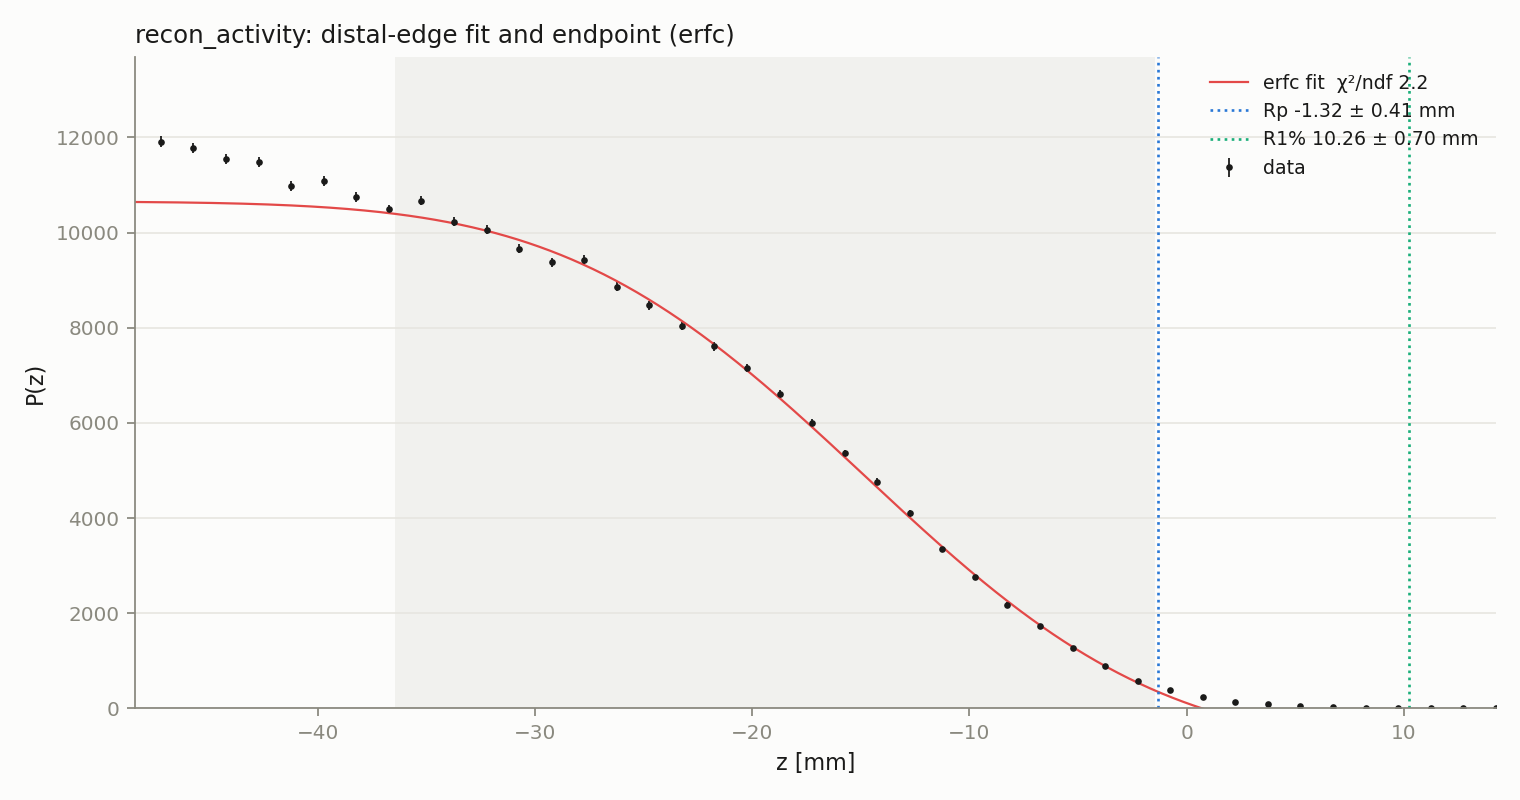
\includegraphics[width=0.9\textwidth]{figs/fit_recon_activity_bgo.png}
  \caption{Whole-plane depth profile of one reconstructed \SI{1}{Gy} BGO
    acquisition (points, Poisson errors) and the erfc fit
    (Eq.~\ref{eq:erfc}, red line) in the fixed window (shaded). The
    markers show two derived points: the tangent endpoint $R_p$ and the
    1\% crossing.}
  \label{fig:fit}
\end{figure}

\section{Calibration budgets}
\label{sec:budget}

Each stage of the measurement chain shifts $\DR$ by a definite, resolvable
amount, and the decomposition is measured per arm over its ten independent
acquisitions (Table~\ref{tab:ladder}, Fig.~\ref{fig:ladder}): from the true
activity to the origins of the detected true coincidences (the acceptance
stage: attenuation and solid-angle weighting), to the MLEM reconstruction
of the trues, to the reconstruction of \emph{all} events with no scatter or
randoms correction.

\begin{table}[htb]
  \centering
  \caption{The calibration budgets: $\DR$ at each rung of the measurement
    chain (erfc fit), over each arm's ten \SI{1}{Gy} acquisitions ---
    mean $\pm$ standard error, [acquisition-to-acquisition spread]. The
    truth-level value, common to both, is \SI{-10.743}{mm}.}
  \label{tab:ladder}
  \vspace{1mm}
  \begin{tabular}{lll}
    \toprule
    rung & {BGO 195\,K [mm]} & {CsI [mm]} \\
    \midrule
    detected trues (origins) & $-10.938 \pm 0.007$~~[0.023]
                             & $-10.962 \pm 0.012$~~[0.039] \\
    reconstruction (trues)   & $-11.165 \pm 0.020$~~[0.065]
                             & $-11.232 \pm 0.027$~~[0.084] \\
    reconstruction (all events, uncorrected)
                             & $-11.144 \pm 0.036$~~[0.113]
                             & $-11.192 \pm 0.036$~~[0.114] \\
    \bottomrule
  \end{tabular}
\end{table}

\begin{figure}[htb]
  \centering
  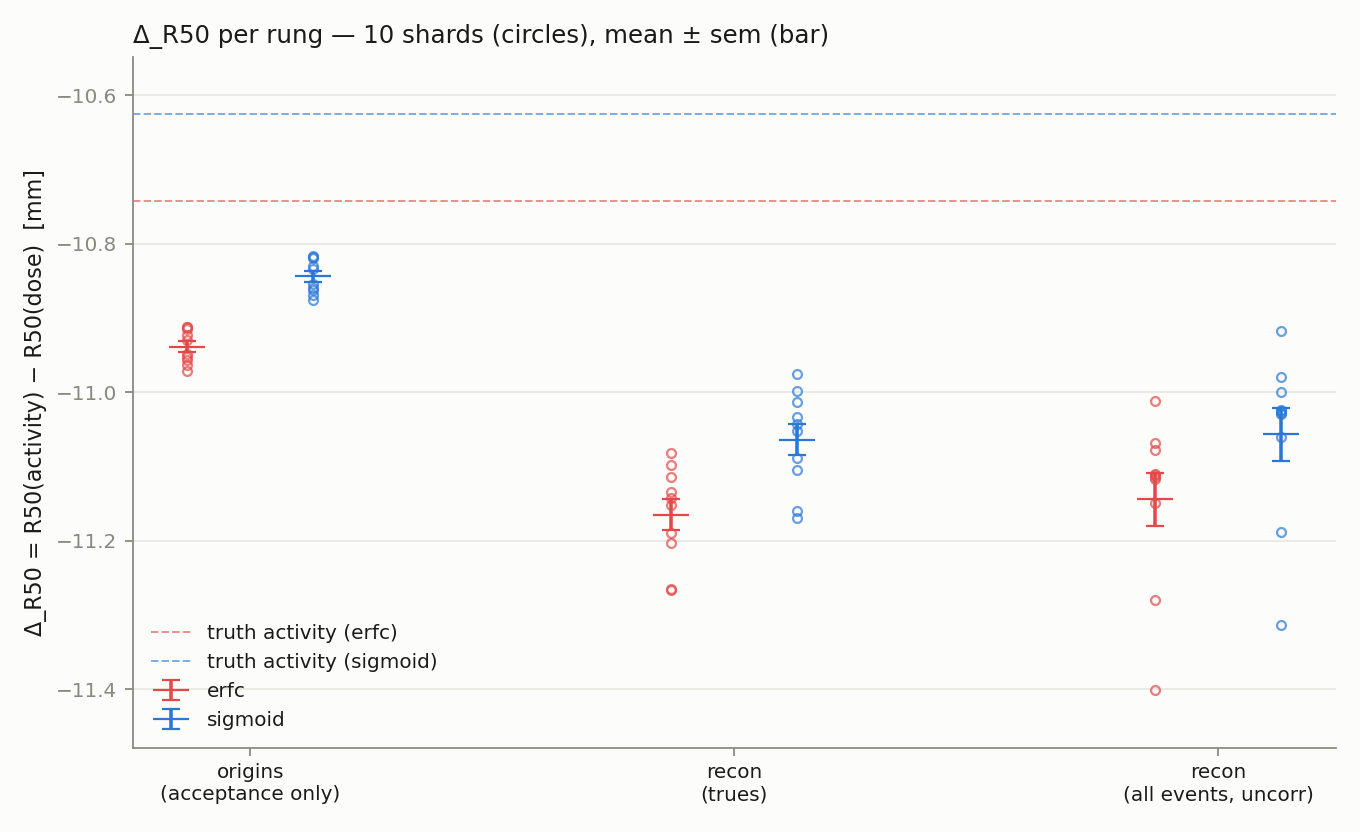
\includegraphics[width=0.49\textwidth]{figs/ladder_delta_r50_bgo.png}
  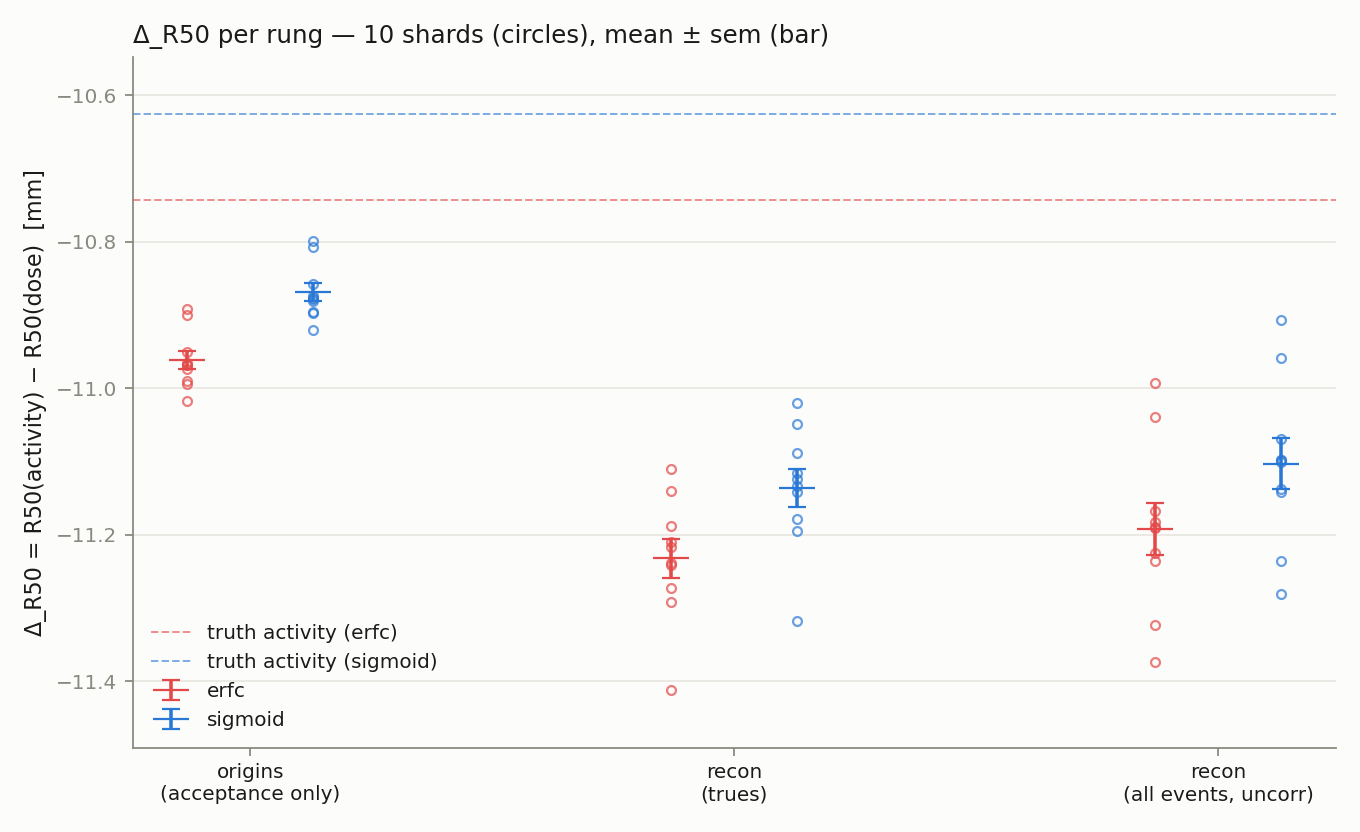
\includegraphics[width=0.49\textwidth]{figs/ladder_delta_r50_csi.png}
  \caption{$\DR$ per rung for the ten acquisitions (circles) with mean
    $\pm$ sem (bars), for the erfc (red) and logistic (blue) fits; the
    dashed lines are the truth-level values. Left: BGO 195\,K; right: CsI.}
  \label{fig:ladder}
\end{figure}

The budgets read the same on both arms: the acceptance stage moves the
edge by ${\sim}\SI{-0.2}{mm}$, the reconstruction by a further
${\sim}\SI{-0.25}{mm}$, and admitting the scattered and random
coincidences uncorrected changes it by $+0.021$ (BGO) and
$+\SI{0.040}{mm}$ (CsI). Each term is a constant of the chain that the
per-scanner reference simulation calibrates, measured here to
\SIrange{0.01}{0.04}{mm} --- far below the effects the verification aims
to detect.

The precision is quoted as the spread over independent acquisitions ---
the fluctuation a real measurement has. (The per-fit errors on
reconstructed profiles are conservative by a factor $\approx 2.5$, a known
consequence of the correlations MLEM introduces between neighbouring
voxels; on the origins rung, where the counts are honestly Poisson, the
per-fit error matches the spread.)

\section{The two arms tie --- and why}
\label{sec:tie}

Table~\ref{tab:k} is the central result. On true coincidences BGO's
$2.1\times$ statistics buys the expected $\sqrt{N}$ advantage. Admitting
the uncorrected event mix --- the protocol a real scanner runs --- costs
BGO a factor $1.7$ in spread against CsI's $1.4$, and the two arms land on
the same number:
\begin{equation}
  \sigma_R(\SI{1}{Gy},\ \text{all events})
  \;=\; 0.113 \pm 0.027\ \text{(BGO 195\,K)}
  \quad\text{vs.}\quad 0.114 \pm \SI{0.029}{mm}\ \text{(CsI)}.
\end{equation}

\begin{table}[htb]
  \centering
  \caption{The scanner constants: $\sigma_R$ at \SI{1}{Gy} from each arm's
    ten acquisitions (erfc, whole-plane). The all-events row is the
    realistic protocol; the trues row is what a perfect scatter correction
    would recover.}
  \label{tab:k}
  \vspace{1mm}
  \begin{tabular}{lcc}
    \toprule
    selection & BGO 195\,K & CsI \\
    \midrule
    true coincidences  & $\SI{0.065 \pm 0.015}{mm}$ & $\SI{0.084 \pm 0.020}{mm}$ \\
    all events, uncorrected & $\SI{0.113 \pm 0.027}{mm}$ & $\SI{0.114 \pm 0.029}{mm}$ \\
    \bottomrule
  \end{tabular}
\end{table}

The mechanism is instructive. The scattered coincidences do not bias the
edge --- the shifts in Table~\ref{tab:ladder} are \SIrange{0.02}{0.04}{mm},
because the scatter background reconstructs into a smooth dome under the
edge (Fig.~\ref{fig:scatters}) whose gentle window slope the free baseline
of Eq.~(\ref{eq:erfc}) absorbs (worst-case bounds $-0.13$ and
\SI{-0.28}{mm}; measured $+0.02$ and $+\SI{0.04}{mm}$). What they add is
\emph{variance}: mispositioned events that fluctuate acquisition to
acquisition without sharpening the edge. Purity and statistics are
therefore exchangeable at this protocol, and the two representative
crystals happen to exchange them at par.

The corollary sets the agenda: \textbf{a scatter correction is the
tiebreaker}. Recovering the trues-level precision is worth a factor $1.7$
to BGO and $1.4$ to CsI (Table~\ref{tab:k}), so the correction --- or a
tighter selection exploiting CsI's energy resolution --- is where the
technology comparison will be decided.

\begin{figure}[htb]
  \centering
  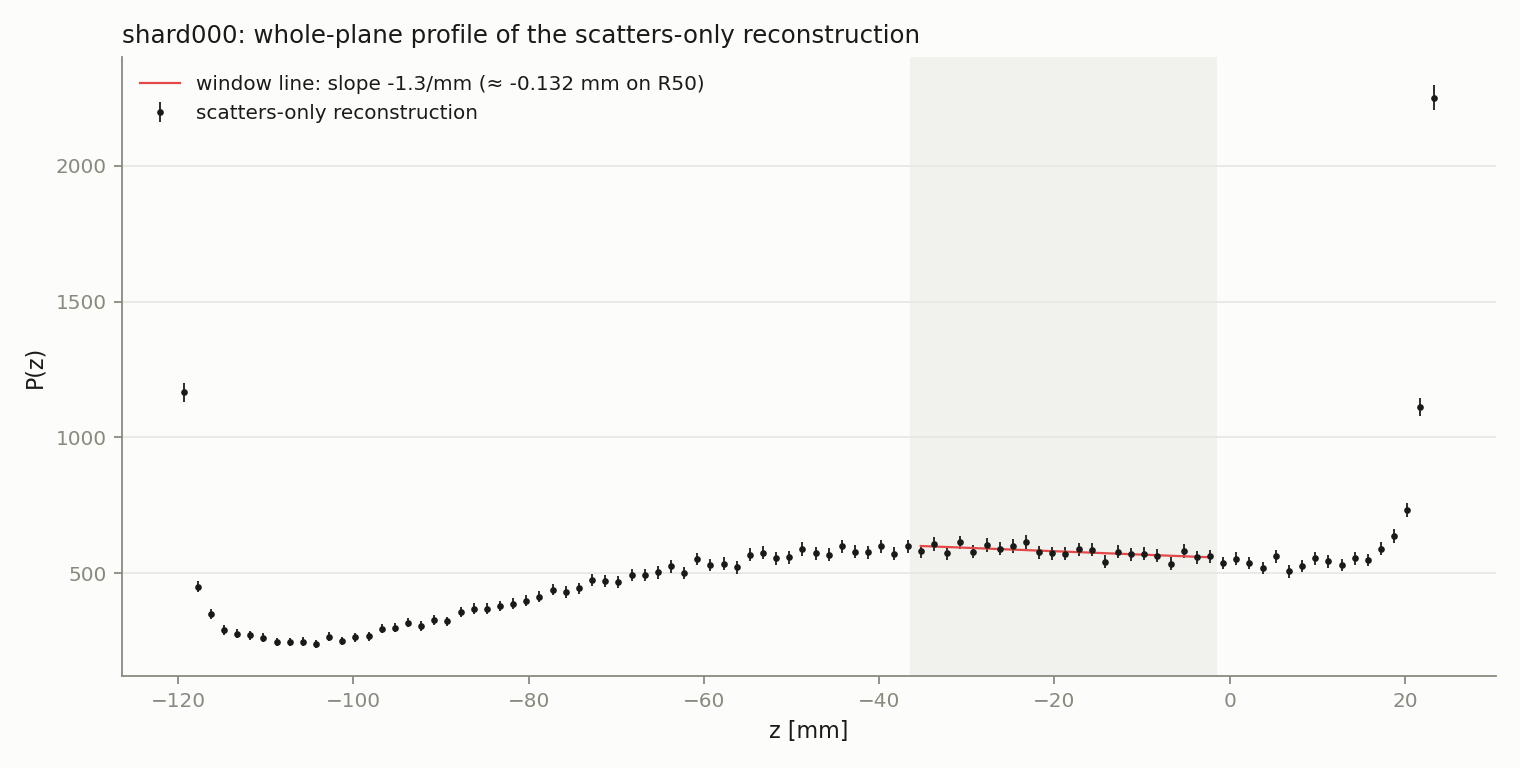
\includegraphics[width=0.49\textwidth]{figs/scatters_profile_bgo.png}
  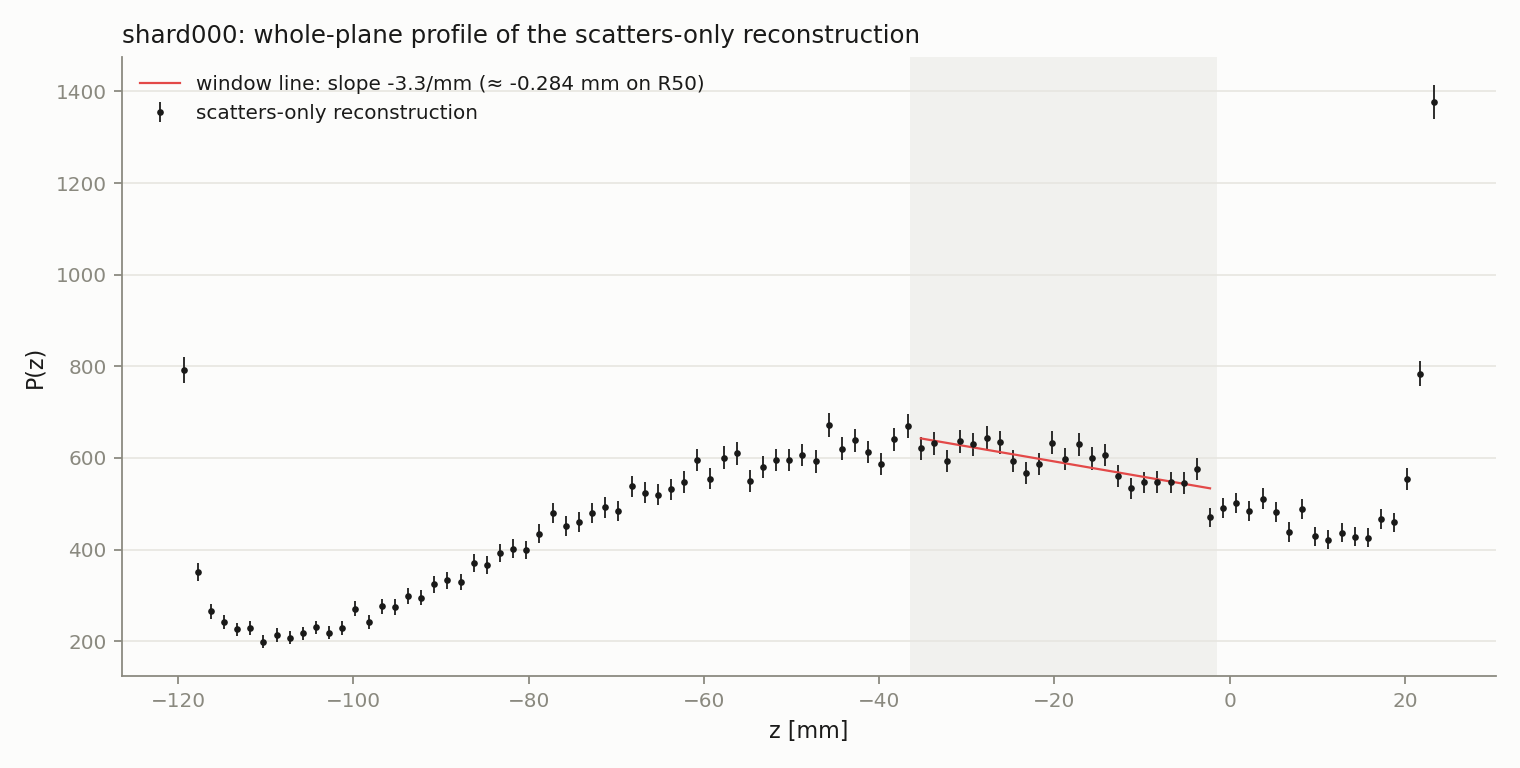
\includegraphics[width=0.49\textwidth]{figs/scatters_profile_csi.png}
  \caption{Whole-plane profile of the scatters-only reconstruction of one
    acquisition, in the units of the joint (all-events) image: BGO 195\,K
    (left, $27.4\%$ of events) and CsI (right, $13.3\%$). The red line is
    a straight fit inside the window; its slope bounds the worst-case
    effect on $\Rfifty$.}
  \label{fig:scatters}
\end{figure}

\section{Low-dose operation}
\label{sec:dose}

The dose axis is explored by thinning each stored acquisition with the
appropriate Bernoulli probability and reconstructing each realisation with
the identical chain. Figure~\ref{fig:dose} shows $\DR$ for every
realisation, grouped by dose, and the measured $\sigma_R$ against the
$1/\sqrt{\text{dose}}$ law anchored at \SI{1}{Gy}; Table~\ref{tab:dose}
quantifies the two operating points per arm (true coincidences).

\begin{table}[htb]
  \centering
  \caption{The two operating points per arm (erfc fit, whole-plane
    profile, trues). $n$ is the number of independent realisations.}
  \label{tab:dose}
  \vspace{1mm}
  \begin{tabular}{llS[table-format=2]S[table-format=-2.3]S[table-format=1.3]S[table-format=1.3]S[table-format=1.3]}
    \toprule
    arm & {dose [Gy]} & {$n$} & {$\DR$ [mm]} & {sem [mm]}
      & {$\sigma_R$ [mm]} & {$\pm$ [mm]} \\
    \midrule
    BGO 195\,K & 1.0 & 10 & -11.165 & 0.020 & 0.065 & 0.015 \\
    BGO 195\,K & 0.1 & 20 & -11.192 & 0.036 & 0.159 & 0.026 \\
    CsI        & 1.0 & 10 & -11.232 & 0.027 & 0.084 & 0.020 \\
    CsI        & 0.1 & 20 & -11.198 & 0.051 & 0.230 & 0.037 \\
    \bottomrule
  \end{tabular}
\end{table}

\begin{figure}[htb]
  \centering
  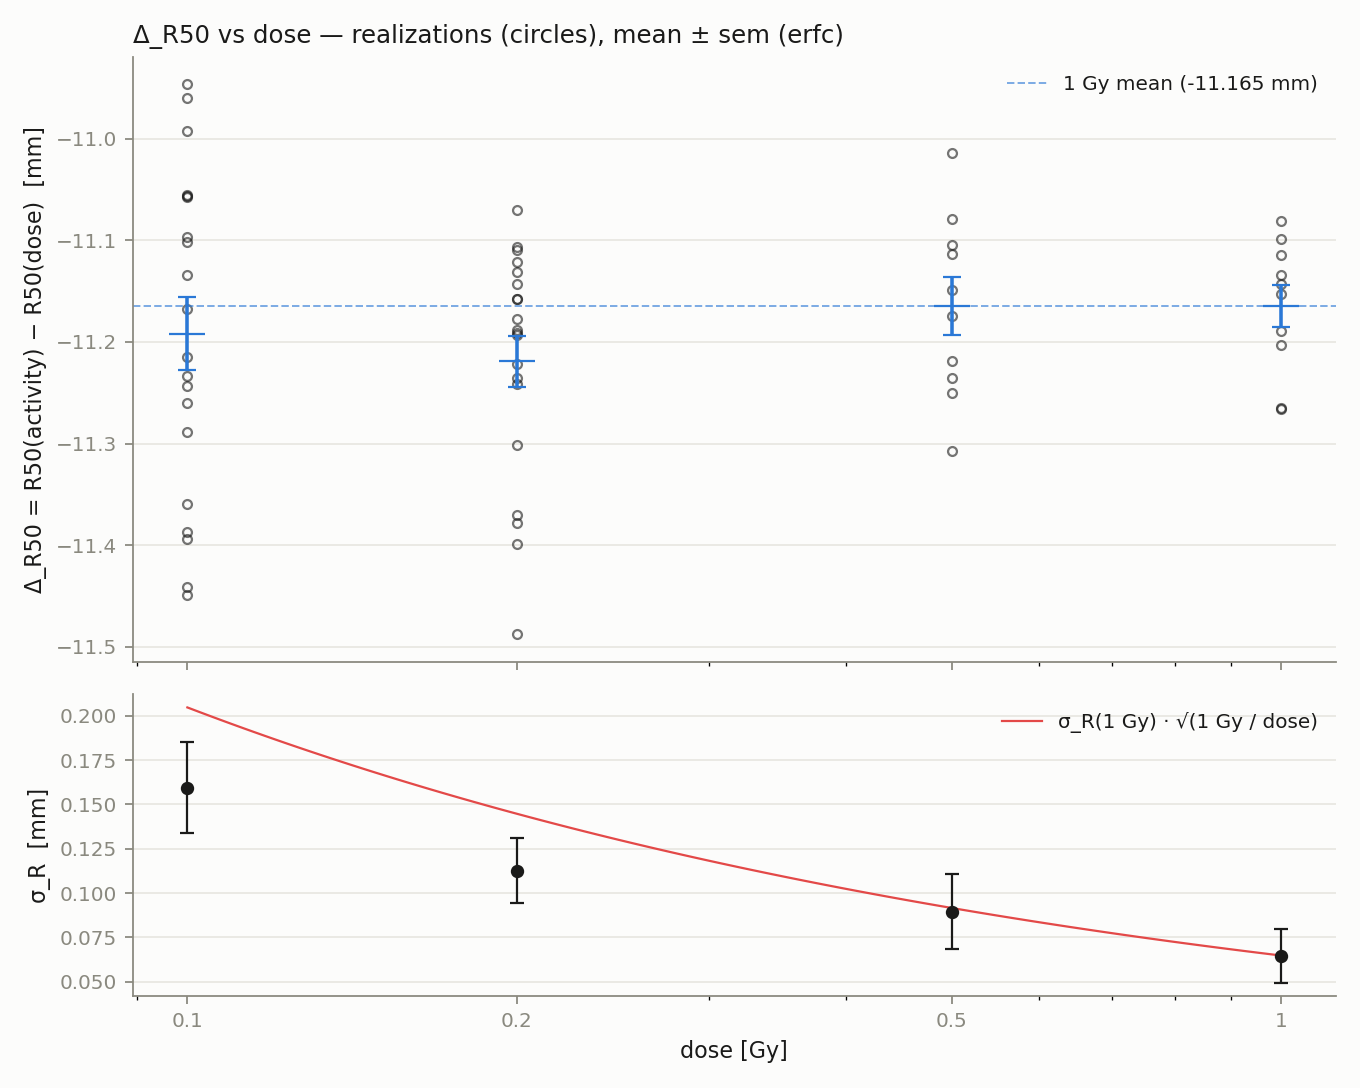
\includegraphics[width=0.49\textwidth]{figs/dose_sweep_r50_bgo.png}
  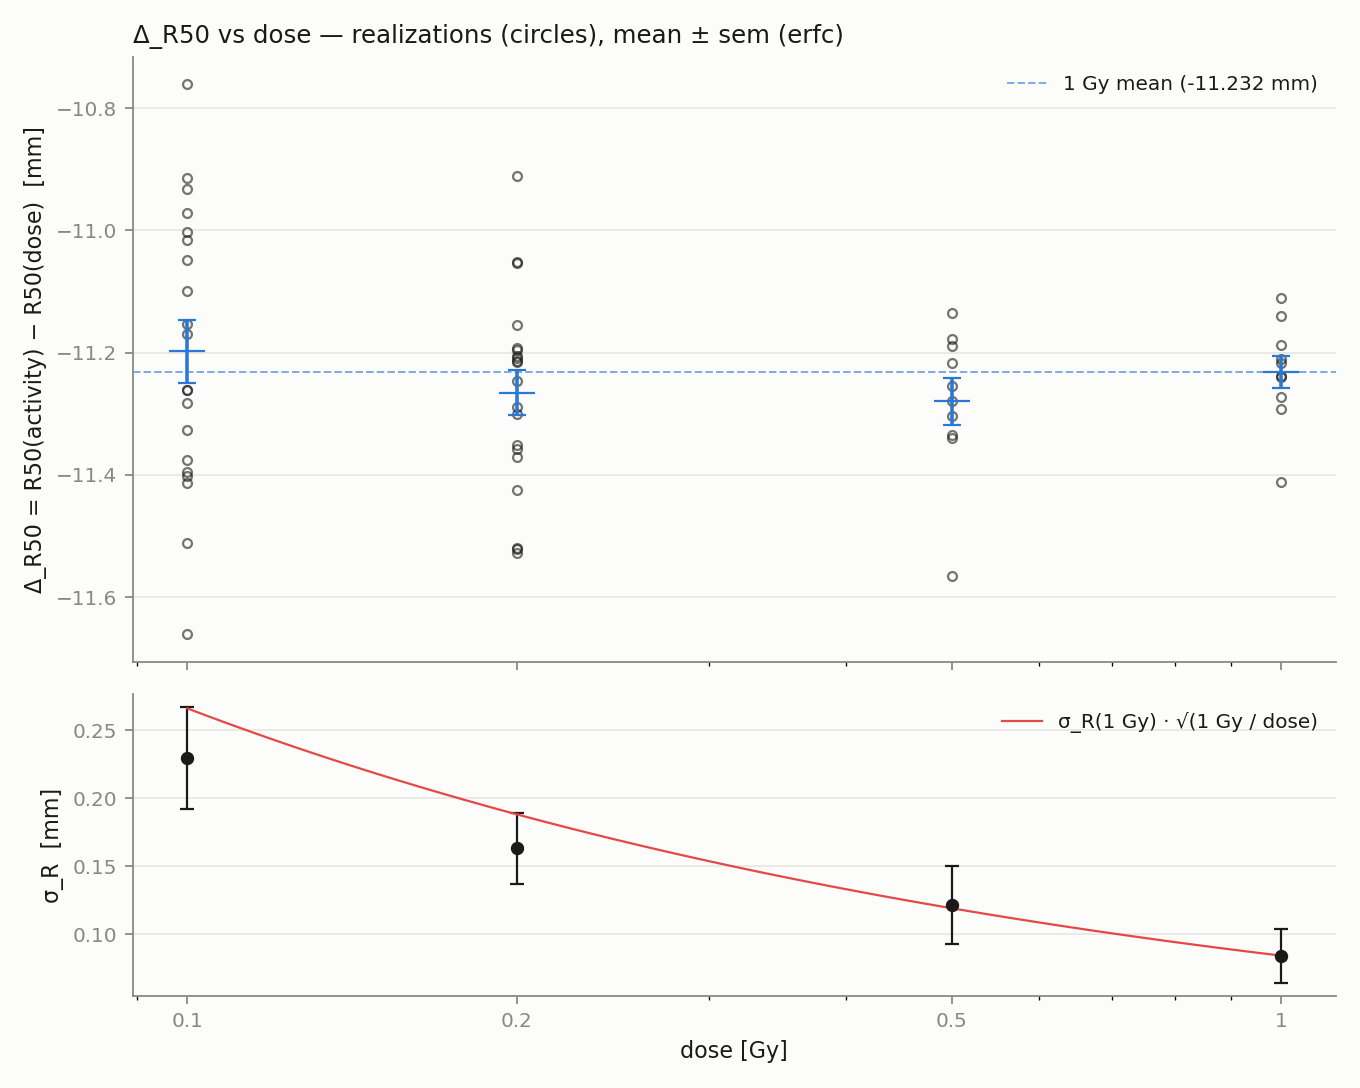
\includegraphics[width=0.49\textwidth]{figs/dose_sweep_r50_csi.png}
  \caption{Top panels: $\DR$ for every realisation (circles) grouped by
    dose, with mean $\pm$ sem; the dashed line is the \SI{1}{Gy} mean.
    Bottom panels: the spread $\sigma_R$ per dose against the
    $1/\sqrt{\text{dose}}$ prediction anchored at \SI{1}{Gy} (red line).
    Left: BGO 195\,K; right: CsI.}
  \label{fig:dose}
\end{figure}

Two facts hold on both arms. The calibration is dose-invariant: the group
means agree with the \SI{1}{Gy} anchor within one standard error down to
\SI{0.1}{Gy} --- the reconstruction places the edge at the same depth over
a factor ten in statistics. And the precision is purely statistical:
$\sigma_R \propto 1/\sqrt{\text{dose}}$ at every measured point, with no
onset of fit instability at low counts.

The consequence is a mode of operation: an \emph{exploratory dose}. A
\SI{0.1}{Gy} shot --- a small fraction of a \SIrange{1}{2}{Gy} daily
fraction --- locates the distal edge with $\sigma_R = 0.16$ (BGO) to
\SI{0.23}{mm} (CsI) and a calibration known to better than \SI{0.05}{mm},
an order of magnitude below the millimetre scale that drives clinical
margins~\cite{paganetti2012}. The beam range can therefore be verified
against the plan before the therapeutic dose is delivered, with the same
scanner and the same analysis.

\section{Outlook}
\label{sec:outlook}

Four directions follow directly from this round.

\paragraph{Scatter correction.} The tiebreaker of
Sec.~\ref{sec:tie}: recovering trues-level precision is worth a factor
$1.7$ (BGO) and $1.4$ (CsI). The scatters-only reconstructions of
Fig.~\ref{fig:scatters} are the input for designing it, and the
per-configuration check (window slope vs.\ edge gradient) is standing.

\paragraph{Acquisition start time.} The isotope activities
(Fig.~\ref{fig:decays}) set the trade-off of in-room imaging: a start
\SIrange{2}{3}{min} after beam-off, rather than one, loses part of the
$^{15}$O signal but shifts the mix towards $^{11}$C, whose positron
endpoint energy (\SI{0.96}{MeV}, against \SI{1.73}{MeV} for $^{15}$O)
carries a correspondingly smaller positron range --- a \emph{sharper}
intrinsic edge. A high-sensitivity scanner can absorb the count loss, so
the delayed start may improve the range measurement rather than degrade
it. The production files carry the absolute decay time of every
coincidence, so any start time is a pure event selection on the stored
acquisitions --- statistically exact, randoms included.

\paragraph{Isotope-resolved edge model.} The distal fall-off is a
superposition of per-isotope edges with known relative depths. A composite
erfc with simulation-fixed offsets and free amplitudes turns the edge
shape into a measurement of the isotope mix, and is the natural refinement
of Eq.~(\ref{eq:erfc}) for the start-time studies.

\paragraph{Geometry axis.} With the crystal contrast measured, the
remaining scanner axes --- ring length (sensitivity) and open geometries
(angular coverage) --- run through the identical battery; the analysis is
configuration-blind by construction.

\begin{figure}[htb]
  \centering
  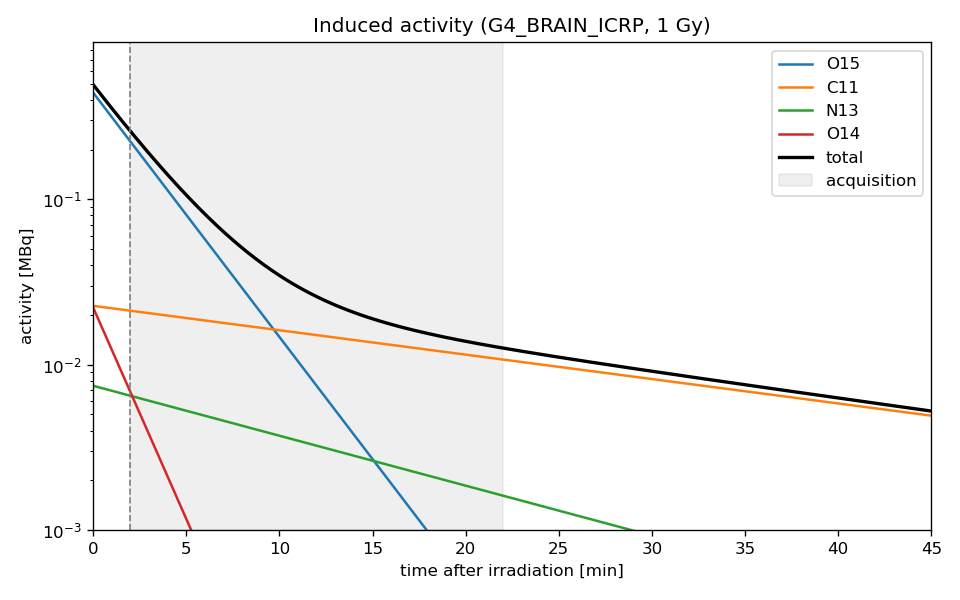
\includegraphics[width=0.8\textwidth]{figs/activity.png}
  \caption{Activity of the $\beta^+$ emitters produced by the field, as a
    function of time: the currency of the acquisition-start trade-off.}
  \label{fig:decays}
\end{figure}

\section*{Conclusions}

The whole-plane erfc fit of the $\beta^+$ depth profile, with $\Rfifty$ as
the range observable and the activity--dose offset calibrated per scanner
on the reference simulation, is a robust distal-edge estimator: its
conventions contribute below \SI{0.1}{mm}, its calibration budget is
measured to \SIrange{0.01}{0.04}{mm} per term on both arms, and the
scattered coincidences bias it by no more than \SI{0.04}{mm} without
correction. The first technology round is a tie: BGO 195\,K and cryogenic
CsI both measure the distal edge with $\sigma_R = \SI{0.11}{mm}$ per
\SI{1}{Gy} acquisition at the uncorrected protocol --- statistics against
purity, at par. The trues-level precisions ($0.065$ vs.\ \SI{0.084}{mm})
state what a scatter correction would unlock on each arm, making that
correction the deciding question of the comparison. On both arms the
precision scales as $1/\sqrt{\text{dose}}$ with a dose-invariant
calibration, so an exploratory \SI{0.1}{Gy} shot verifies the beam range
to \SIrange{0.16}{0.23}{mm} before the clinical dose is delivered.

\bibliographystyle{unsrtnat}
\bibliography{biblio}

\end{document}
